\noindent The code implementation of the registration function is shown in Fig.\ref{png1}. It first validates the user by requesting the \texttt{username} and the \texttt{password} from the user. The password must be 6-20 characters. After the validation, if the current user is not in the database, a new entry for the user will be created in the database user table with \texttt{create}. An ID is assigned to the user with \texttt{rand} function. After a successful registration, it will automatically jump to the login interface.

% The report must be at most 12,000 words or 35 pages (whichever is less)?超级爱你 我也爱你哦�� xin❤️xi��xin❤x❤️xi❤️❤️❤️nixnxin

\begin{figure}[H]
  \centering
  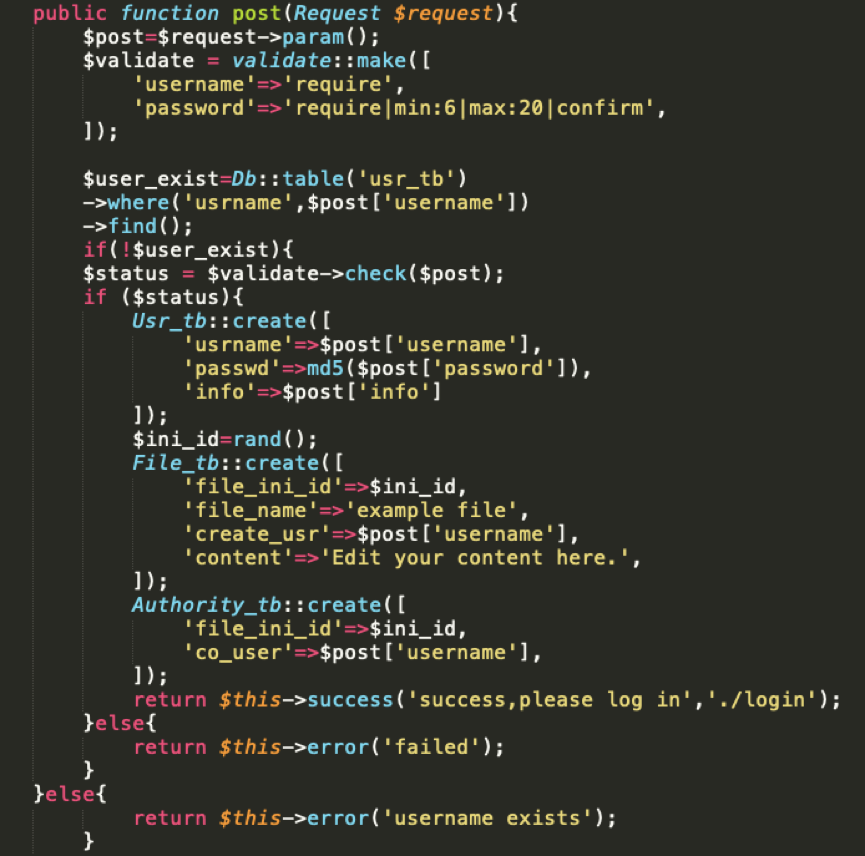
\includegraphics[width=.8\textwidth]{register.png} %图片文件的相对路径
  \caption{Code snippet of the registration function} %caption是图片的标题
  \label{png1} %此处的label相当于一个图片的专属标志,目的是方便上下文的引用
\end{figure}


\noindent The code implementation of the login function is shown in Fig.\ref{png2}. It first uses \texttt{IF} function to determine whether the user name received is the same as the username retrieved from the database. Then,the password is encrypted with \texttt{MD5} and the cipher text,which will be compared with the corresponding cipher in the session. Once the session values are equal, the user is verified to be successfully login and jumps automatically to the main web page(index.html).
\begin{figure}[H]
  \centering
  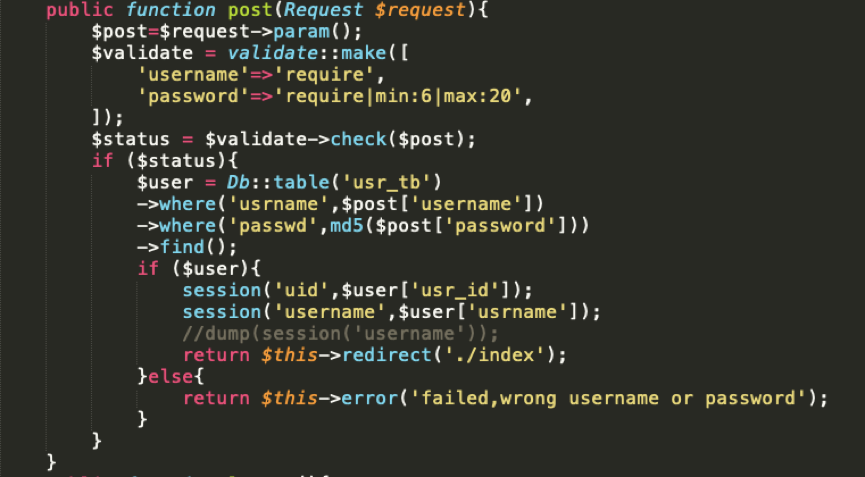
\includegraphics[width=.8\textwidth]{login.png} %图片文件的相对路径
  \caption{Code snippet of the login function} %caption是图片的标题
  \label{png2} %此处的label相当于一个图片的专属标志,目的是方便上下文的引用
\end{figure}

\noindent The code implementation of the file creation function is shown in Fig.\ref{png3}. It first generate and allocate file id by using \texttt{rand},then the database allocates space to this new file as well as update the permissions in the authority table.
\begin{figure}[H]
  \centering 
  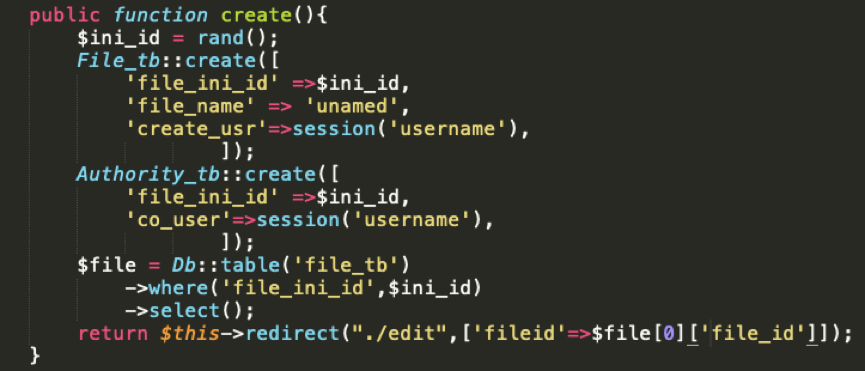
\includegraphics[width=.8\textwidth]{createfile.png} %图片文件的相对路径
  \caption{Code snippet of the file creation function} %caption是图片的标题
  \label{png3} %此处的label相当于一个图片的专属标志,目的是方便上下文的引用
\end{figure}



\noindent The code implementation of the file upload function is shown in Fig.\ref{png4}.The function of this code is to upload the existing local file to the database in the server.In detail,first and the most,it use the \texttt{IF}function to restrict the file type and size.After getting the local file path and extracting the contents of the file with \texttt{file\_get\_contents},it also randomly generates \texttt{file\_id}for the file.Finally, all the information relate to this file will be stored into the database.
\begin{figure}[H]
  \centering
  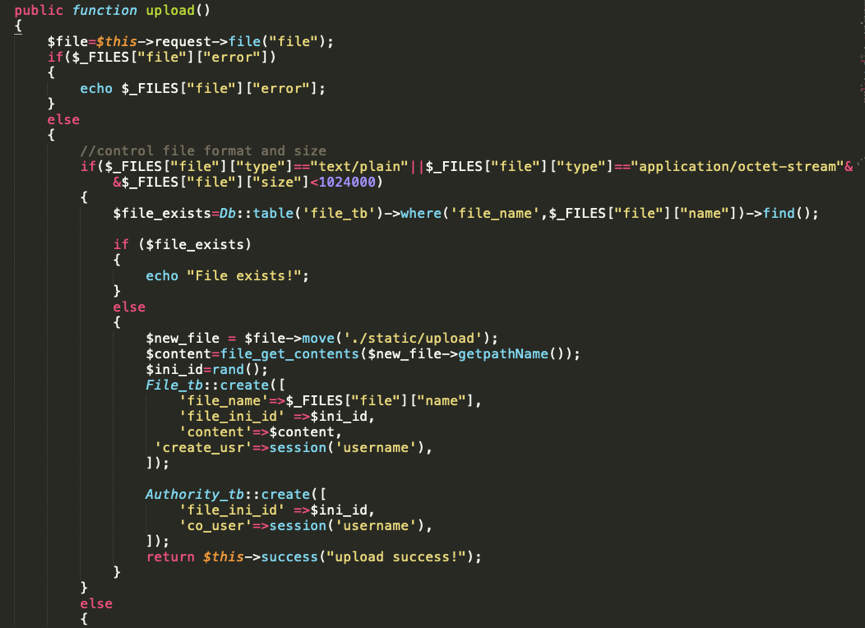
\includegraphics[width=.8\textwidth]{upnowfile.png} %图片文件的相对路径
  \caption{Code snippet of the file upload function} %caption是图片的标题
  \label{png4} %此处的label相当于一个图片的专属标志,目的是方便上下文的引用
\end{figure}


\noindent The code implementation of the file edit function is shown in Fig.\ref{png5}.In this edit interface, click \texttt{upload} to enter this function. Determine if there is a version error, if it does not exist, update the data to the database; if it exists, insert the data into the database and enter the compare page.

\begin{figure}[H]
  \centering
  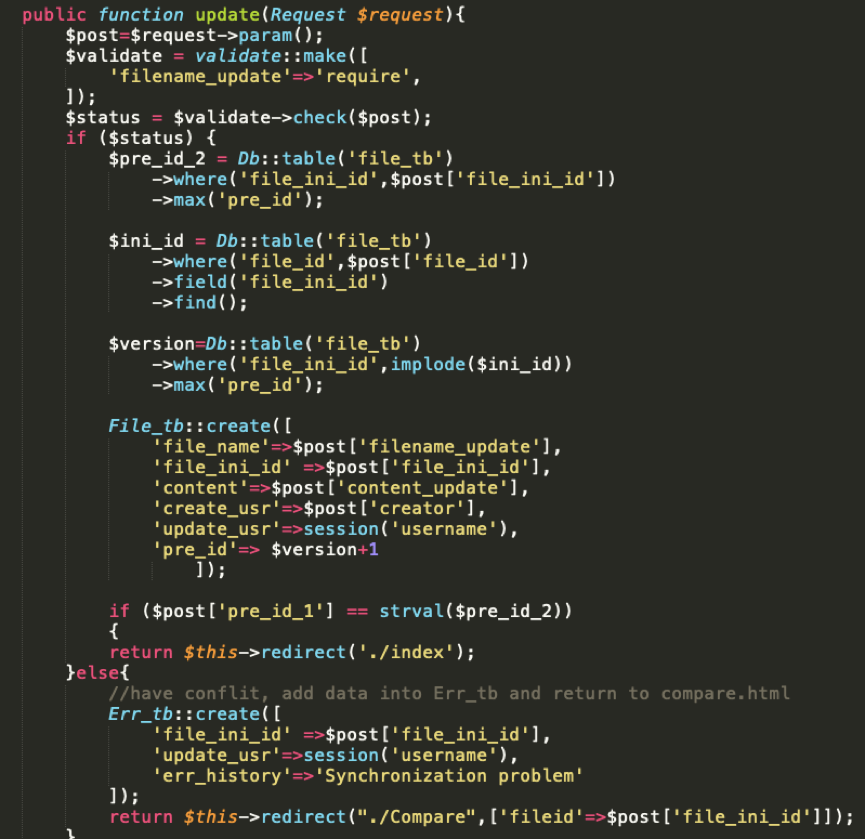
\includegraphics[width=.8\textwidth]{edit.png} %图片文件的相对路径
  \caption{Code snippet of the file edit function} %caption是图片的标题
  \label{png5} %此处的label相当于一个图片的专属标志,目的是方便上下文的引用
\end{figure}


\noindent The code implementation of adding coordinator function is shown in Fig.\ref{png6}.After determining whether there is a \texttt{username} to be added in \texttt{co\_user}, the system will operate differently depending on the particular case. If the coordinator already exists in database, it will not be added. If it does not exist, add this user into the permission table.
\begin{figure}[H]
  \centering
  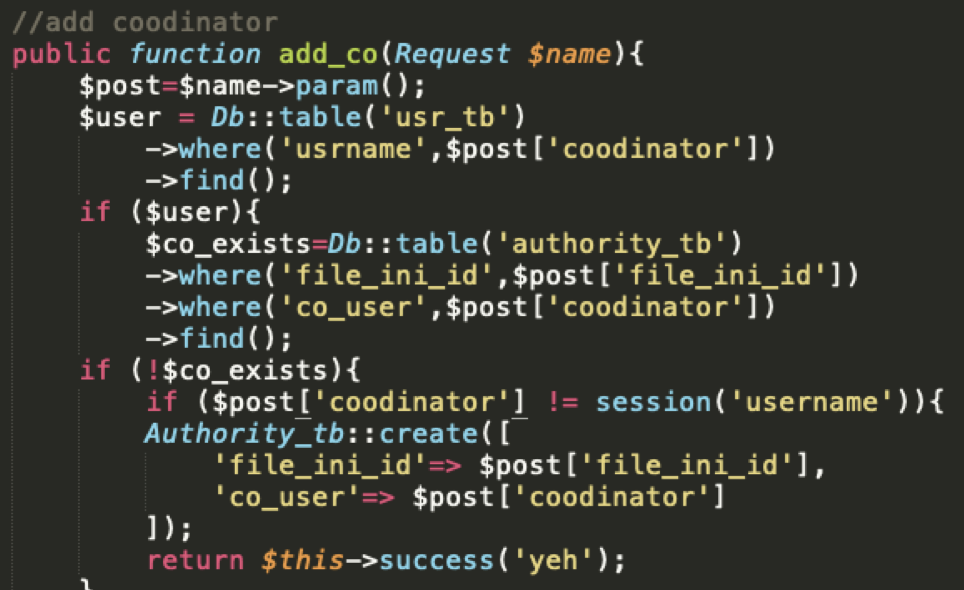
\includegraphics[width=.8\textwidth]{addco.png} %图片文件的相对路径
  \caption{Code snippet of adding coordinator function} %caption是图片的标题
  \label{png6} %此处的label相当于一个图片的专属标志,目的是方便上下文的引用
\end{figure}

\noindent The code implementation of Frontend modification permission function is shown in Fig.\ref{png7}.First, the if statement is used to determine that only the creator of the file will have the add and delete buttons. We can delete the edit authentication by their \texttt{username}.
\begin{figure}[H]
  \centering
  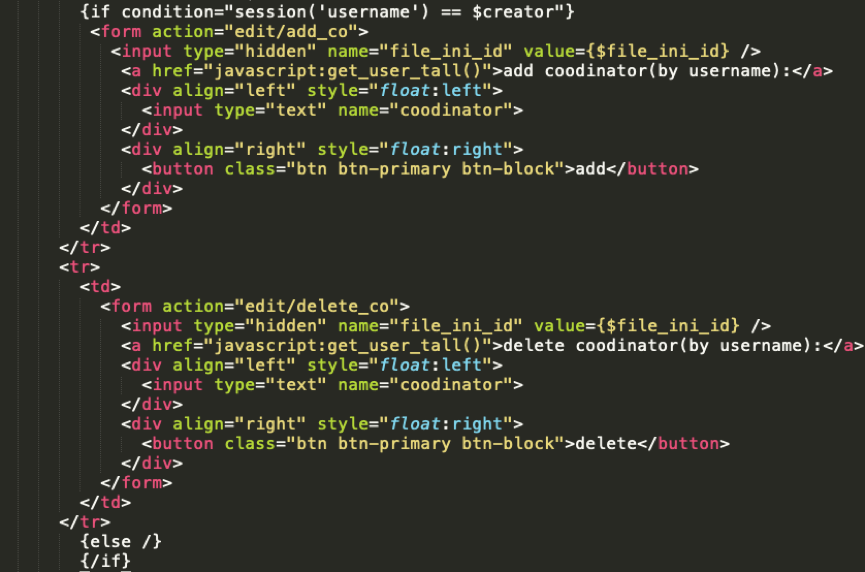
\includegraphics[width=.8\textwidth]{qianduan.png} %图片文件的相对路径
  \caption{} %caption是图片的标题
  \label{png7} %此处的label相当于一个图片的专属标志,目的是方便上下文的引用
\end{figure}



\noindent The code implementation of checking and returning to the historical version function is shown in Fig.\ref{png8}.
\begin{figure}[H]
  \centering
  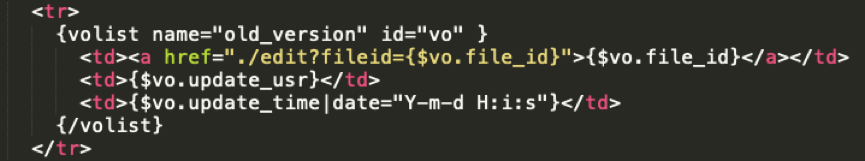
\includegraphics[width=.8\textwidth]{changeback.png} %图片文件的相对路径
  \caption{Code snippet of checking and returning to the historical version} %caption是图片的标题
  \label{png8} %此处的label相当于一个图片的专属标志,目的是方便上下文的引用
\end{figure}


\noindent The code implementation of checking and solving conflicts are shown separately in Fig.\ref{png9}.and Fig.\ref{png10}.This moment it have already encountered a conflict. According to the solution we designed, we need to construct a comparison page to compare the two conflicting documents together,and then, select the required version as the latest version according to the situation.
\noindent It gets the id of the file by using the \texttt{GET} command, then uses \texttt{fetch} to send the name and content of the two files to the compare page.
\noindent In the compare interface, the user can clearly see the contents of the two files and manually determine the version they want to keep, then they can choose to save this version of the file as the latest version.The code snippet in Fig.\ref{png10} is an example of saving the previous version of the file. After resetting the file\_id by \texttt{redirect}, it will automatically return to the index page.
\begin{figure}[H]
  \centering
  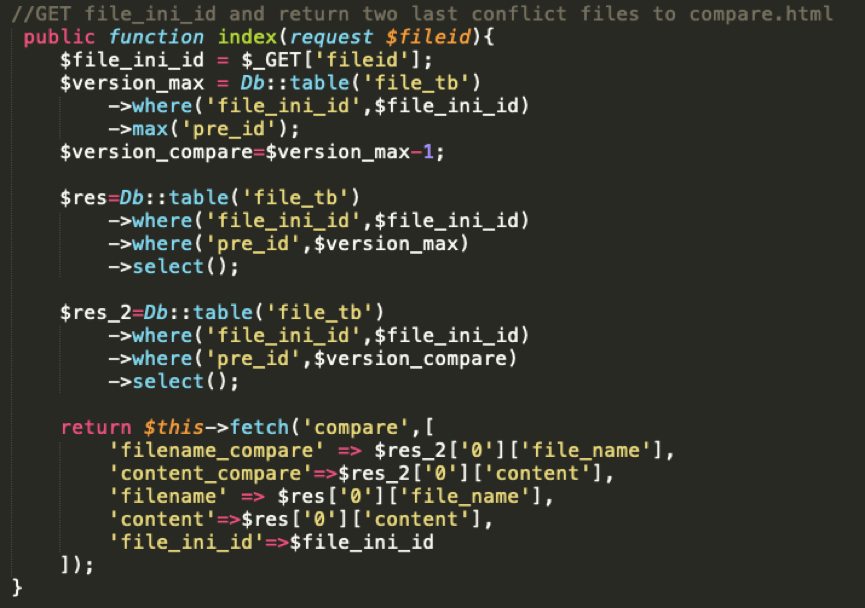
\includegraphics[width=.8\textwidth]{conflict.png}%图片文件的相对路径
  \caption{Code snippet of checking conflicts} %caption是图片的标题
  \label{png9} %此处的label相当于一个图片的专属标志,目的是方便上下文的引用
\end{figure}

\begin{figure}[H]
  \centering
  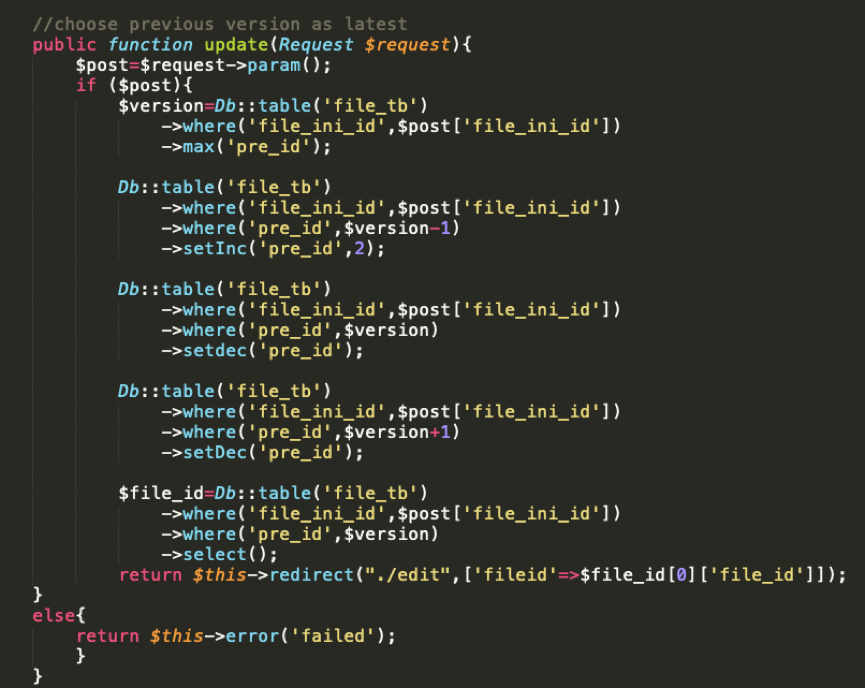
\includegraphics[width=.8\textwidth]{conflictsolve.png}%图片文件的相对路径
  \caption{Code snippet of saving the previous version} %caption是图片的标题
  \label{png10} %此处的label相当于一个图片的专属标志,目的是方便上下文的引用
\end{figure}

